\chapter{Discussion}\label{chapter:discussion}

One aim of the master thesis was to investigate whether a micro-frontend architecture with GraphQL using a shared caching layer and query reduction can improve performance. The improvement should be accomplished using a single caching layer for all micro-frontends and a mechanism to reduce queries by utilizing the in-memory cache structure. The technology-agnostic implementation of the caching strategy is further discussed in this chapter. The results of evaluating the caching improvements of the prototypical micro-frontend implementation architecture are also discussed in this chapter. The findings of Chapter \ref{chapter:results} are used to make a statement about the hypothesis from Chapter \ref{section:introduction:hypothesis}. The following sections focus on discussing the results regarding request size and response size. The chapter closes by comparing the total times to fetch all responses from the GraphQL \ac{API}.

\section{Request Size}\label{section:discussion:request-size}

This section compares the different measurements of the request sizes from Chapter \ref{chapter:results}. Figure \ref{fig:discussion:request-size} displays the results from the previous sections \ref{section:results:comparison-first-journey} and \ref{section:results:comparison-second-journey} as a bar chart for better comparison. As can be seen from the figure for the first user journey, the differences in request sizes are not very large. The first approach without query reduction and a separate cache is the largest and executes 11 more GraphQL queries than the other two. These 11 extra GraphQL queries make up the total difference from the second approach with the shared caching layer since the queries are not reduced using the cache. The difference between the second and third approach is only 1.65 KB, which is quite insignificant.

\bigskip

\noindent The second user journey shows a similar result. Compared to the first, 25 requests are omitted in the second approach by just using a shared caching layer. These differences in the number of network requests results in a greater difference in request sizes, about 6.07 KB. However, the difference from the second approach to the third approach is slight, as it is again about 2.17 KB. The difference between the second and third approach comes only from the reduced fields in a query. The difference of 2.17 KB is relatively tiny compared to the 37 GraphQL queries that were executed against the \ac{BFF}.

\bigskip

\noindent Therefore, the query reduction functionality does not significantly improve performance by reducing the size of the responses compared to just using the shared caching layer.

\ifshowImages
\begin{figure}[H]
  \centering
  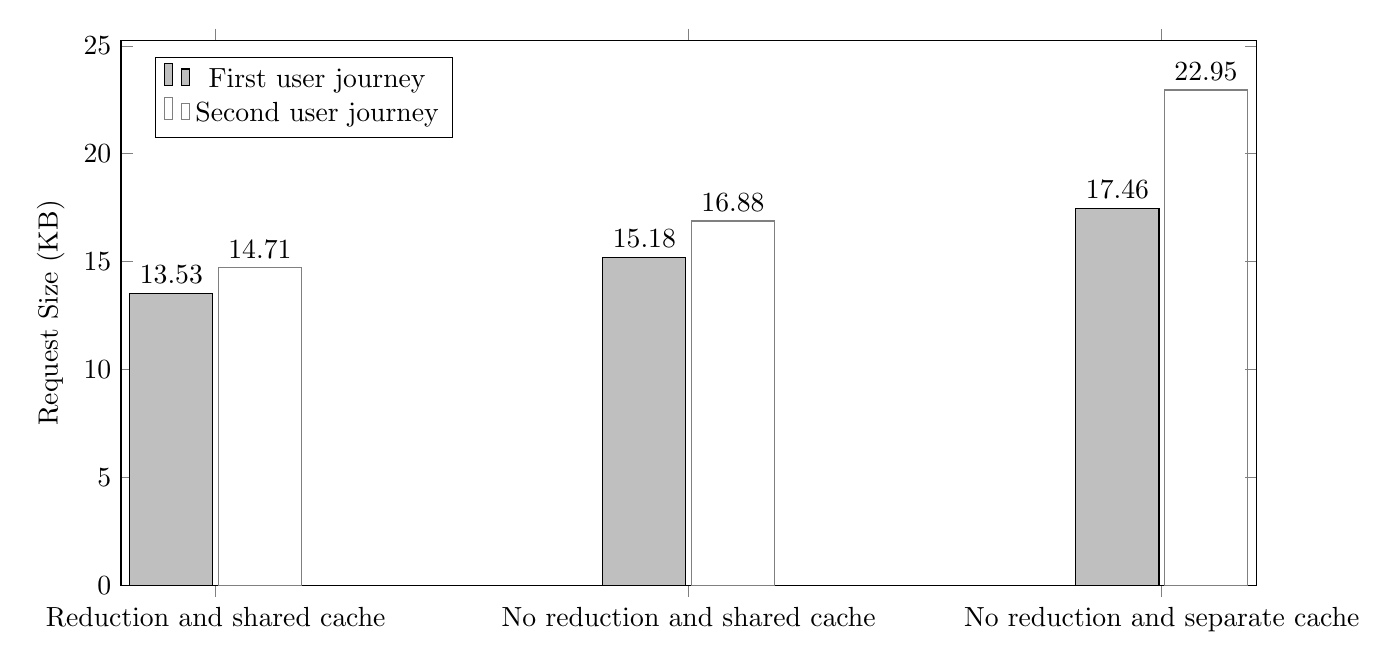
\begin{tikzpicture}
    \begin{axis}[
      ymin=0,
      ybar,
      legend pos=north west,
      ylabel={Request Size (KB)},
      xtick=data, 
      symbolic x coords={Reduction and shared cache, No reduction and shared cache, No reduction and separate cache}, 
      nodes near coords align={vertical},
      nodes near coords,
      height=8.5cm,
      width=16cm,
      bar width=30pt,
      cycle list={
        {fill=lightgray, draw=gray}
      },
    ]
    \addplot coordinates {(Reduction and shared cache, 13.53) (No reduction and shared cache, 15.18) (No reduction and separate cache, 17.46)};
    \addplot coordinates {(Reduction and shared cache, 14.71) (No reduction and shared cache, 16.88) (No reduction and separate cache, 22.95)};
    \legend{First user journey, Second user journey}
    \end{axis}
  \end{tikzpicture}
  \caption{Request size comparison between the three approaches.}\label{fig:discussion:request-size}
\end{figure}
\fi

\noindent The following section compares the response sizes of the GraphQL \ac{API} for the three approaches.

\section{Response Size}\label{section:discussion:response-size}

This section compares the three approaches' response sizes from the GraphQL \ac{API}. Figure \ref{fig:discussion:response-size} displays the results already shown in the previous sections \ref{section:results:comparison-first-journey} and \ref{section:results:comparison-second-journey} as a bar chart for better comparison. Clearly, visible is that the differences in response size are more significant than the difference in request size. As displayed in the figure, the difference between the first approach and the others is more than 2 MB. Therefore, the 11 requests that are omitted by using a shared caching layer are responsible for more than 2 MB of data that is downloaded unnecessarily. This difference can significantly affect the performance of the page when using a mobile device. The difference between the second and third approach is only about 62 KB, which is insignificant and does not make a real difference. Saving 62 KB of data in 37 GraphQL queries is not worth the effort of maintaining and using the query reduction functionality. 

\bigskip

\noindent The second user journey shows a similar outcome, as the size differences are almost identical. Using the second approach in the user journey eliminates 25 queries compared to the naive first approach. These fewer requests result again in a difference of about 2.35 MB. The second and third approach have just a 3 KB difference in response sizes. These differences are coming solely from the reduced fields of GraphQL queries, which are pretty small compared to the 37 GraphQL queries that are executed against the \ac{BFF}.

\bigskip

\noindent Just like with the request sizes, query reduction does not significantly improve performance by reducing the size of the network responses compared to just using the shared caching layer.

\ifshowImages
\begin{figure}[H]
  \centering
  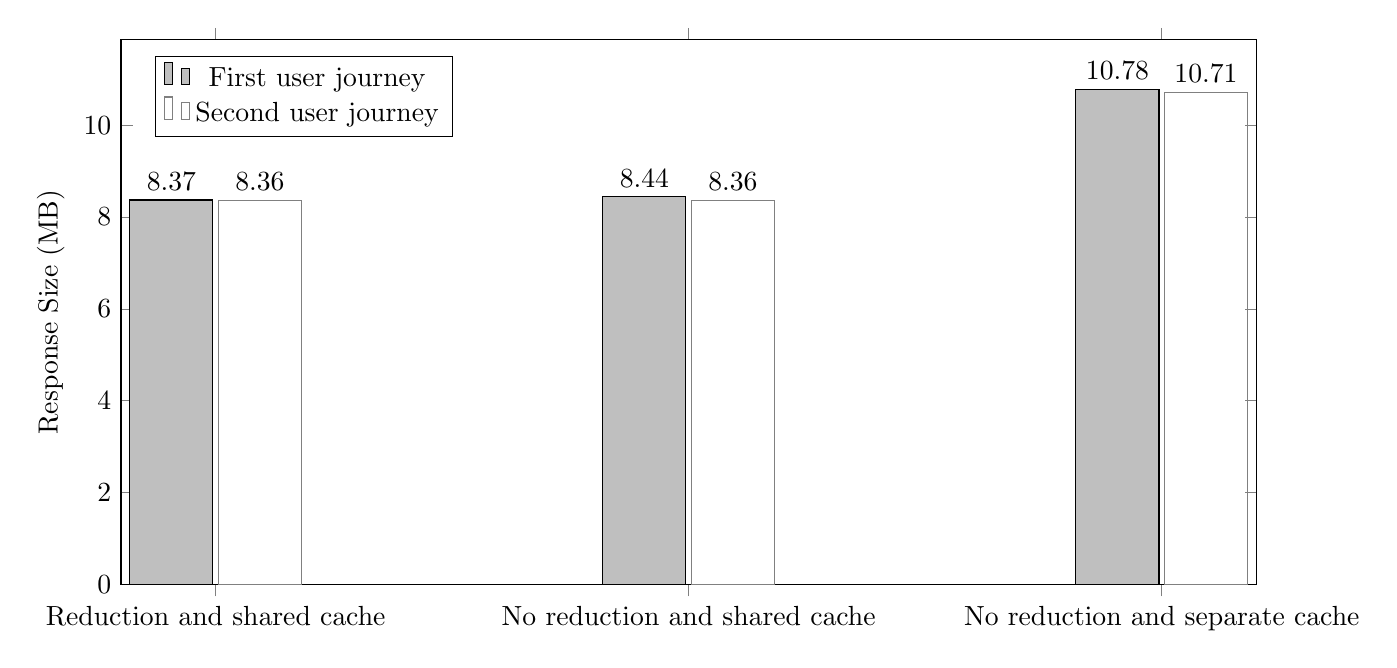
\begin{tikzpicture}
    \begin{axis}[
      ymin=0,
      ybar,
      legend pos=north west,
      ylabel={Response Size (MB)},
      xtick=data, 
      symbolic x coords={Reduction and shared cache, No reduction and shared cache, No reduction and separate cache}, 
      nodes near coords align={vertical},
      nodes near coords,
      height=8.5cm,
      width=16cm,
      bar width=30pt,
      cycle list={
        {fill=lightgray, draw=gray}
      },
    ]
    \addplot coordinates {(Reduction and shared cache, 8.37) (No reduction and shared cache, 8.44) (No reduction and separate cache, 10.78)};
    \addplot coordinates {(Reduction and shared cache, 8.361) (No reduction and shared cache, 8.364) (No reduction and separate cache, 10.71)};
    \legend{First user journey, Second user journey}
    \end{axis}
  \end{tikzpicture}
  \caption{Response size comparison between the three approaches.}\label{fig:discussion:response-size}
\end{figure}
\fi

\noindent The following section compares the response times of the three approaches. This factor is vital because smaller responses lead to faster page loads, which is crucial for the user experience.

\section{Response Time}\label{section:discussion:response-times}

It is hard to make accurate comparisons when it comes to measuring the time it takes to fetch the responses from a GraphQL \ac{API}. The network speed can vary significantly over time; therefore, it takes some time to make a reproducible comparison. Therefore, the measurement was done using the throttle mode inside the Google DevTools\footnote{\url{https://developer.chrome.com/docs/devtools/}}. The network speed was set to 1.5 Mbps, also named \enquote{fast 3G} preset inside the developer tools. This setting ensures the network speed stays the same for testing all three approaches. The response times were measured three times for every approach, and the mean value was taken to get a neutral value. The preset \enquote{fast 3G} was chosen because it is pretty slow and makes it possible to compare the measurements better. With faster network speeds, the differences would be more minor and harder to compare. Moreover, 3G is still a typical network speed for mobile connections in many countries.

\bigskip

\noindent This section compares the total time to download every query response from the GraphQL \ac{API} for the three approaches from Section \ref{section:results:performance-measurement}. The measurement should not be misunderstood, because the browser typically loads the resources in parallel. Here, only the total download time is measured to see how much time it takes to download all the resources in one of the approaches. The measurements were recorded during the user journeys from sections \ref{section:results:comparison-first-journey} and \ref{section:results:comparison-second-journey} alongside the request sizes and response sizes. Therefore the total response times correspond to the measured network sizes from the previous two sections. The results are measured in seconds and are shown in Figure \ref{fig:discussion:response-times}. 

\ifshowImages
\begin{figure}[H]
  \centering
  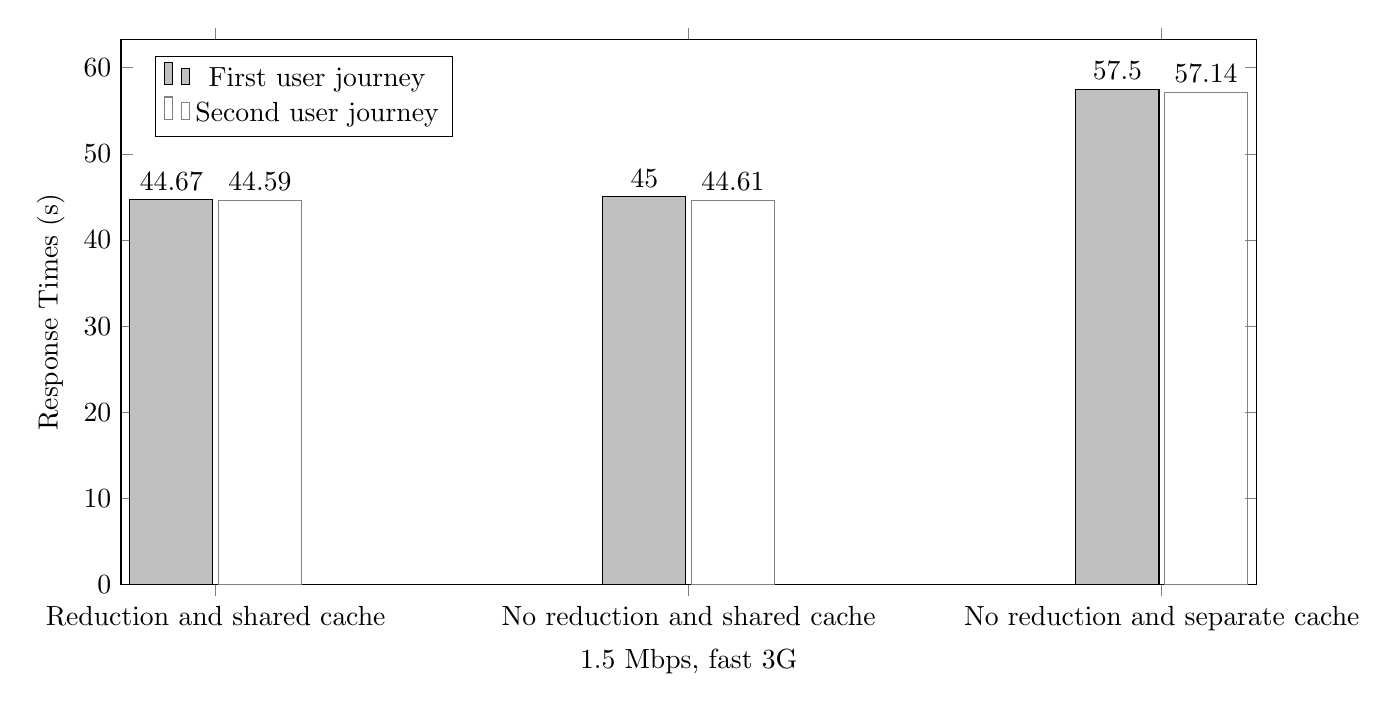
\begin{tikzpicture}
    \begin{axis}[
      ymin=0,
      ybar,
      legend pos=north west,
      ylabel={Response Times (s)},
      xlabel={1.5 Mbps, fast 3G},
      xtick=data, 
      symbolic x coords={Reduction and shared cache, No reduction and shared cache, No reduction and separate cache}, 
      nodes near coords align={vertical},
      nodes near coords,
      height=8.5cm,
      width=16cm,
      bar width=30pt,
      cycle list={
        {fill=lightgray, draw=gray}
      },
    ]
    \addplot coordinates {(Reduction and shared cache, 44.67) (No reduction and shared cache, 45.00) (No reduction and separate cache, 57.50)};
    \addplot coordinates {(Reduction and shared cache, 44.59) (No reduction and shared cache, 44.61) (No reduction and separate cache, 57.14)};
    \legend{First user journey, Second user journey}
  \end{axis}
  \end{tikzpicture}
  \caption{Response time comparison between the three approaches.}\label{fig:discussion:response-times}
\end{figure}
\fi

\noindent Like before, the difference between the first and second approach is quite significant. The second approach is about 12 seconds faster than the first approach for both journeys. The 11, respectively, 25 requests omitted using the shared caching layer are responsible for about 12 seconds of extra download time for the first approach. The results for the second and third approach are practically the same. The results for the second and third approaches are virtually identical. The reduction of 37 queries does not lead to the expected results and does not argue for the use of query reduction.